\trilingualchapter{Food Service Operations: The Heart of the Restaurant}{餐饮服务运营:餐厅的核心}{Lebensmittelservice: Das Herz des Restaurants}{}

The kitchen and dining room are where the restaurant concept comes to life. This chapter delves into menu development, kitchen operations, service standards, and the daily rhythm of food service that Sue and Owen established at their Artisan Bistro.

\section{Menu Development | 菜单开发 | Menüentwicklung}

The menu is the restaurant's primary communication tool with customers. Sue and Owen spent months developing a menu that reflected their concept, supported their business model, and delighted their guests.

\subsection{Menu Philosophy}

Their menu philosophy centered on:
\begin{itemize}
    \item \textbf{Seasonality}: Using ingredients at their peak
    \item \textbf{Local sourcing}: Supporting regional producers
    \item \textbf{Technique}: Traditional methods with modern touches
    \item \textbf{Balance}: Variety in flavors, textures, and price points
    \item \textbf{Executability}: Dishes that can be consistently executed
\end{itemize}

\subsection{Menu Structure | 菜单结构 | Menüstruktur}

\subsubsection{Menu Categories}
\begin{itemize}
    \item \textbf{Appetizers}: Small plates to start the meal
    \item \textbf{Soups and Salads}: Lighter options
    \item \textbf{Entrées}: Main courses (meat, seafood, vegetarian)
    \item \textbf{Sides}: Accompaniments
    \item \textbf{Desserts}: Sweet endings
    \item \textbf{Beverages}: Wine, beer, cocktails, non-alcoholic
\end{itemize}

\subsubsection{Menu Engineering}

Sue and Owen used menu engineering to optimize profitability:

\begin{table}[h]
\centering
\begin{tabular}{lcccc}
\toprule
\textbf{Item} & \textbf{Popularity} & \textbf{Profit Margin} & \textbf{Category} & \textbf{Action} \\
\midrule
Braised Short Rib & High & High & Star & Promote \\
Grilled Salmon & High & Low & Plowhorse & Reprice/Reduce cost \\
Lamb Chops & Low & High & Puzzle & Reposition/Promote \\
Vegetable Risotto & Low & Low & Dog & Remove/Revise \\
\bottomrule
\end{tabular}
\caption{Menu Engineering Matrix}
\end{table}

\subsection{Menu Pricing | 菜单定价 | Menüpreisgestaltung}

\subsubsection{Pricing Strategies}
\begin{itemize}
    \item \textbf{Cost-plus pricing}: Food cost × multiplier (typically 3-4×)
    \item \textbf{Competitive pricing}: Based on market rates
    \item \textbf{Value-based pricing}: Based on perceived value
    \item \textbf{Psychological pricing}: \$19.95 vs \$20.00
\end{itemize}

\subsubsection{Pricing Considerations}
\begin{itemize}
    \item Target food cost percentage (28-35\%)
    \item Labor costs
    \item Overhead allocation
    \item Competitive positioning
    \item Customer price sensitivity
    \item Profit margin goals
\end{itemize}

\subsection{Menu Design and Presentation | 菜单设计与呈现 | Menüdesign und Präsentation}

\begin{itemize}
    \item Clear, readable typography
    \item Logical organization
    \item Descriptive but not overwhelming
    \item Highlight signature dishes
    \item Accommodate dietary restrictions (vegetarian, gluten-free, etc.)
    \item Update regularly to reflect availability
\end{itemize}

\section{Kitchen Operations | 厨房运营 | Küchenbetrieb}

\subsection{Kitchen Organization | 厨房组织 | Küchenorganisation}

\begin{figure}[h]
\centering
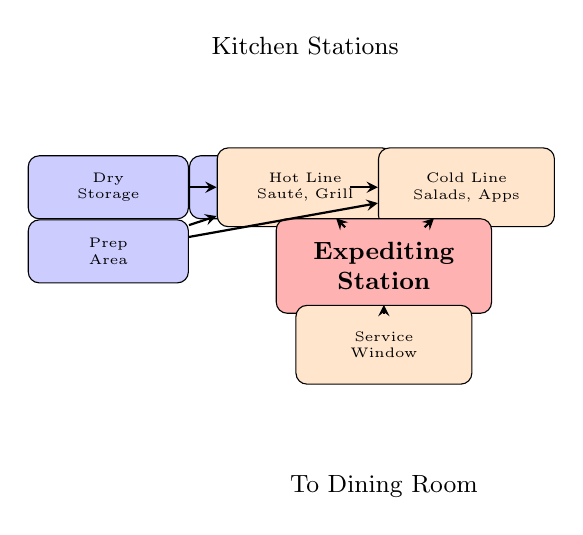
\begin{tikzpicture}[
    node distance=1.5cm,
    auto,
    station/.style={rectangle, draw, fill=orange!20, text width=2cm, text centered, rounded corners, minimum height=1cm, font=\tiny},
    expedite/.style={rectangle, draw, fill=red!30, text width=2.5cm, text centered, rounded corners, minimum height=1.2cm, font=\small\bfseries},
    storage/.style={rectangle, draw, fill=blue!20, text width=1.8cm, text centered, rounded corners, minimum height=0.8cm, font=\tiny},
    arrow/.style={thick,->,>=stealth}
]
    % Storage areas
    \node [storage, above left] (dry) {Dry\\Storage};
    \node [storage, above right] (cold) {Cold\\Storage};
    \node [storage, below left] (prep) {Prep\\Area};
    
    % Kitchen stations
    \node [station, right of=dry, xshift=1cm] (hot) {Hot Line\\Sauté, Grill};
    \node [station, right of=cold, xshift=1cm] (coldline) {Cold Line\\Salads, Apps};
    \node [expedite, below of=hot, yshift=0.5cm, xshift=1cm] (exp) {Expediting\\Station};
    
    % Service
    \node [station, below of=exp, yshift=0.5cm] (service) {Service\\Window};
    
    % Arrows
    \draw [arrow] (dry) -- (hot);
    \draw [arrow] (cold) -- (coldline);
    \draw [arrow] (prep) -- (hot);
    \draw [arrow] (prep) -- (coldline);
    \draw [arrow] (hot) -- (exp);
    \draw [arrow] (coldline) -- (exp);
    \draw [arrow] (exp) -- (service);
    
    % Labels
    \node [above of=hot, yshift=0.3cm, font=\small] {Kitchen Stations};
    \node [below of=service, yshift=-0.3cm, font=\small] {To Dining Room};
\end{tikzpicture}
\caption{Kitchen Layout and Flow}
\label{fig:kitchen_layout}
\end{figure}

\subsubsection{Kitchen Brigade}

Sue and Owen organized their kitchen using a modified brigade system:

\begin{itemize}
    \item \textbf{Executive Chef} (Sue): Menu development, quality control
    \item \textbf{Sous Chef}: Day-to-day operations, training
    \item \textbf{Line Cooks}: Hot line, cold line, grill
    \item \textbf{Prep Cooks}: Mise en place, preparation
    \item \textbf{Dishwasher}: Cleaning, basic prep support
\end{itemize}

\subsubsection{Station Organization}

\begin{itemize}
    \item \textbf{Hot line}: Sauté, grill, fry
    \item \textbf{Cold line}: Salads, appetizers, desserts
    \item \textbf{Expediting}: Order coordination, plating, quality check
    \item \textbf{Prep area}: Off-peak preparation
\end{itemize}

\subsection{Standard Operating Procedures (SOPs) | 标准操作程序 (SOPs) | Standardbetriebsverfahren (SOPs)}

Sue and Owen documented SOPs for consistency:

\subsubsection{Preparation Procedures}
\begin{itemize}
    \item Mise en place standards
    \item Prep lists and timing
    \item Quality standards for each item
    \item Storage and labeling
    \item Cross-contamination prevention
\end{itemize}

\subsubsection{Cooking Procedures}
\begin{itemize}
    \item Recipe standardization
    \item Cooking temperatures and times
    \item Plating specifications
    \item Holding times and temperatures
    \item Quality checkpoints
\end{itemize}

\subsection{Food Safety | 食品安全 | Lebensmittelsicherheit}

\subsubsection{HACCP Principles}

Hazard Analysis Critical Control Points:
\begin{enumerate}
    \item Conduct hazard analysis
    \item Identify critical control points
    \item Establish critical limits
    \item Monitor procedures
    \item Corrective actions
    \item Verification procedures
    \item Record keeping
\end{enumerate}

\subsubsection{Key Safety Practices}
\begin{itemize}
    \item Temperature monitoring (receiving, storage, cooking, holding)
    \item Proper handwashing (frequent, thorough)
    \item Cross-contamination prevention (separate cutting boards, utensils)
    \item Time and temperature control (danger zone: 40-140°F)
    \item Proper cooling procedures
    \item Cleaning and sanitizing schedules
\end{itemize}

\subsection{Kitchen Efficiency | 厨房效率 | Kücheneffizienz}

\subsubsection{Workflow Optimization}
\begin{itemize}
    \item Logical station placement
    \item Minimize movement
    \item Equipment accessibility
    \item Clear communication systems
    \item Efficient plating areas
\end{itemize}

\subsubsection{Time Management}
\begin{itemize}
    \item Prep schedules (morning, afternoon, evening)
    \item Batch preparation
    \item Par levels for prepared items
    \item Service timing coordination
\end{itemize}

\section{Service Operations | 服务运营 | Servicebetrieb}

\subsection{Service Standards | 服务标准 | Servicestandards}

Sue and Owen established clear service standards:

\subsubsection{Service Philosophy}
\begin{itemize}
    \item Warm, genuine hospitality
    \item Anticipate guest needs
    \item Knowledgeable about menu and ingredients
    \item Efficient without being rushed
    \item Professional yet approachable
\end{itemize}

\subsubsection{Service Steps}

\begin{enumerate}
    \item \textbf{Greeting}: Warm welcome within 1 minute
    \item \textbf{Seating}: Comfortable, appropriate table
    \item \textbf{Initial contact}: Water, menu presentation, specials
    \item \textbf{Order taking}: Knowledgeable, helpful, accurate
    \item \textbf{Order delivery}: Timing, accuracy, presentation
    \item \textbf{Check-back}: Ensure satisfaction, address needs
    \item \textbf{Payment}: Efficient, friendly
    \item \textbf{Departure}: Thank you, invitation to return
\end{enumerate}

\subsection{Service Staff Organization | 服务人员组织 | Servicepersonalorganisation}

\subsubsection{Service Roles}
\begin{itemize}
    \item \textbf{General Manager} (Owen): Overall operations
    \item \textbf{Service Manager}: Front of house operations
    \item \textbf{Server}: Primary guest contact
    \item \textbf{Bartender}: Bar service, cocktails
    \item \textbf{Host}: Greeting, seating, reservations
    \item \textbf{Busser}: Table maintenance, support
    \item \textbf{Food Runner}: Delivering food from kitchen
\end{itemize}

\subsubsection{Table Management}
\begin{itemize}
    \item Reservation system
    \item Table rotation (fair distribution)
    \item Turn time optimization
    \item Waitlist management
    \item Special requests handling
\end{itemize}

\subsection{Point of Sale (POS) System | 销售点 (POS) 系统 | Kassensystem (POS)}

\subsubsection{POS Functions}
\begin{itemize}
    \item Order entry and transmission
    \item Payment processing
    \item Sales reporting
    \item Inventory tracking
    \item Employee time tracking
    \item Customer data collection
\end{itemize}

\subsubsection{Best Practices}
\begin{itemize}
    \item Accurate order entry
    \item Modifier management
    \item Split checks capability
    \item Tip reporting
    \item Daily reconciliation
\end{itemize}

\section{Quality Control | 质量控制 | Qualitätskontrolle}

\subsection{Quality Standards | 质量标准 | Qualitätsstandards}

\subsubsection{Food Quality}
\begin{itemize}
    \item Consistent execution
    \item Proper temperature
    \item Correct presentation
    \item Fresh ingredients
    \item Proper seasoning
\end{itemize}

\subsubsection{Service Quality}
\begin{itemize}
    \item Timeliness
    \item Accuracy
    \item Professionalism
    \item Knowledge
    \item Problem resolution
\end{itemize}

\subsection{Quality Control Measures | 质量控制措施 | Qualitätskontrollmaßnahmen}

\begin{itemize}
    \item \textbf{Expediting}: Final quality check before service
    \item \textbf{Manager oversight}: Regular floor presence
    \item \textbf{Customer feedback}: Immediate and follow-up
    \item \textbf{Staff training}: Continuous improvement
    \item \textbf{Mystery shoppers}: Objective evaluation
\end{itemize}

\section{Managing Service Flow | 管理服务流程 | Serviceablauf verwalten}

\subsection{Peak Period Management | 高峰期管理 | Spitzenzeitmanagement}

\subsubsection{Preparation}
\begin{itemize}
    \item Adequate staffing
    \item Complete mise en place
    \item Equipment readiness
    \item Communication briefings
\end{itemize}

\subsubsection{During Service}
\begin{itemize}
    \item Clear communication
    \item Efficient workflow
    \item Problem anticipation
    \item Team support
\end{itemize}

\subsection{Handling Challenges | 处理挑战 | Herausforderungen bewältigen}

\subsubsection{Common Issues}
\begin{itemize}
    \item Long wait times
    \item Kitchen delays
    \item Incorrect orders
    \item Unhappy customers
    \item Equipment failures
\end{itemize}

\subsubsection{Resolution Strategies}
\begin{itemize}
    \item Acknowledge issues immediately
    \item Apologize sincerely
    \item Offer solutions
    \item Follow up
    \item Learn and improve
\end{itemize}

\section{Special Events and Catering | 特殊活动与餐饮服务 | Sonderveranstaltungen und Catering}

\subsection{Private Events | 私人活动 | Private Veranstaltungen}

Sue and Owen developed private event capabilities:
\begin{itemize}
    \item Private dining room
    \item Custom menus
    \item Event coordination
    \item Pricing packages
    \item Contract terms
\end{itemize}

\subsection{Catering | 餐饮服务 | Catering}

\begin{itemize}
    \item Off-premise catering
    \item Delivery options
    \item Corporate accounts
    \item Menu adaptation
    \item Logistics planning
\end{itemize}

\section{Continuous Improvement | 持续改进 | Kontinuierliche Verbesserung}

\subsection{Regular Reviews | 定期审查 | Regelmäßige Überprüfungen}

\begin{itemize}
    \item Daily debriefs
    \item Weekly operations meetings
    \item Monthly financial reviews
    \item Quarterly menu reviews
    \item Annual strategic planning
\end{itemize}

\subsection{Feedback Systems | 反馈系统 | Feedbacksysteme}

\begin{itemize}
    \item Customer comment cards
    \item Online reviews monitoring
    \item Staff feedback
    \item Vendor input
    \item Industry trends
\end{itemize}

\trilingualsection{Key Takeaways}{关键要点}{Wichtige Erkenntnisse}{}

\begin{itemize}
    \item Menu is the foundation of operations
    \item Kitchen organization affects efficiency and quality
    \item Food safety is non-negotiable
    \item Service standards create the guest experience
    \item Quality control ensures consistency
    \item Preparation is key to managing peak periods
    \item Continuous improvement drives success
\end{itemize}

With strong food service operations in place, Sue and Owen's restaurant was delivering on its promise. However, none of this would be possible without the right team. The next chapter explores staffing, training, and team development.
